\centerline{\bf \Huge Пересчитаем ребра II}
\centerline{\bf \Huge Решения}

\problem{1}
Дана доска $3 \times 3$. Нарисуйте граф коня для этой доски: то есть граф, вершины которого будут соответствовать клеткам, и две клетки соединены ребром, если они соединены одним ходом коня. Затем перерисуйте этот граф так, чтобы ребра графа на картинке не пересекались.

\textbf{Решение.}
В качестве вершин графа для удобства отметим центры клеток. Нарисуем их зеленым цветом. Ребра графа проведем синим цветом.

\begin{center}
    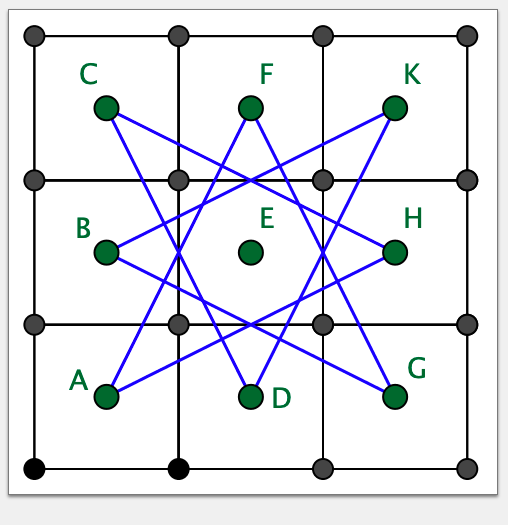
\includegraphics[width=0.4\textwidth]{Сборы/Сборы Элиста 2025/РВ/8/Графы/Решения/g1.png}
\end{center}

Теперь нарисуем вершины по кругу, оставив одну вершину, ни с чем не соединенную, в центре, и соединим вершины ребрами. Обратите внимание на порядок вершин.

\begin{center}
    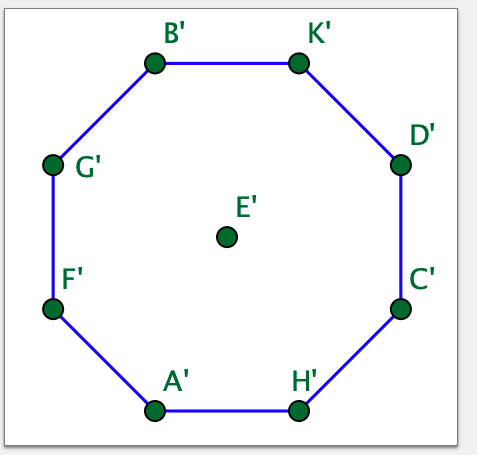
\includegraphics[width=0.4\textwidth]{Сборы/Сборы Элиста 2025/РВ/8/Графы/Решения/g2.png}
\end{center}

\problem{2}
В углах доски $3 \times 3$ стоят кони: по 2 коня черного и белого цветов, причем кони одного цвета стоят в противоположных углах. За один ход разрешается выбрать любого коня и сделать им ход в свободную клетку. Можно ли переставить коней так, чтобы по прежнему все кони стояли в углах, но кони одного цвета стояли в углах при одной стороне?

\textbf{Решение.}
Будем пользоваться рисунком из прошлой задачи. По условию, изначально кони стоят в углах, то есть в вершинах $A, C, K$ и $G$. Пусть не умаляя общности белые кони стоят в вершинах $A$ и $K$, а черные - в $C$ и $G$.
Заметим, что кони могут передвигаться из вершины в вершину только по ребрам. При этом перепрыгивать через вершины они не могут. Значит, порядок коней в этом круге измениться не может. Изначально кони стоят в порядке Белый-Черный-Белый-Черный. Если бы кони одного цвета могли встать в соседних углах, то получился бы порядок Белый-Белый-Черный-Черный. Это, как мы только что выяснили, невозможно, поэтому ответ в задаче — нет, нельзя.

\problem{3}
В королевстве живут графы, герцоги и маркизы. Однажды каждый граф сразился на дуэли с тремя герцогами и несколькими маркизами. Каждый герцог сразился на дуэли с двумя графами и шестью маркизами. Каждый маркиз сразился на дуэли с тремя герцогами и двумя графами. Известно, что все графы сразились с равным числом маркизов. Со сколькими маркизами сразился каждый граф?

\textbf{Решение.}
Пусть каждый граф сразился с $x$ маркизами. Обозначим через $a$ количество графов, через $b$ - количество герцогов, через $c$ - количество маркизов. Заметим, что по условию всего боёв между герцогами и маркизами было с одной стороны $6 b$, а с другой — $3 c$, откуда $c=2 b$. Аналогично посчитаем количество боёв между герцогами и графами двумя способами. Получим $3 a=2 b$. откуда $a=\frac{2}{3} b=\frac{1}{3} c$. Теперь осталось лишь посчитать количество боёв между графами и маркизами двумя способами. Получаем $a x=2 c$, но тогда $\frac{1}{3} c x=2 c$, откуда $x=6$.

\problem{4}
В классе больше 30, но меньше 35 человек. Любой мальчик дружит с тремя девочками, а любая девочка – с пятью мальчиками. Сколько человек в классе?

\textbf{Решение.}
Количество рёбер в соответствующем графе в три раза больше числа мальчиков и в 5 раз больше числа девочек. Следовательно, число девочек относится к числу мальчиков как  3 : 5,  а общее число учеников делится на 8. Между 30 и 35 единственное число делящееся на 8 это 32. 

\problem{5}
В классе 20 учеников, причём каждый дружит не менее, чем с 14 другими. Можно ли утверждать, что найдутся четыре ученика, которые все дружат между собой?

\textbf{Решение.}
Соберём весь класс в одной комнате. Рассмотрим некоторого человека $A$. Пусть теперь из комнаты выйдут все ученики, которые не дружат с $A$. По условию таких не более пяти. Поэтому в комнате осталось по крайней мере 15 учеников. Выберем из оставшихся в комнате ученика $B$, отличного от $A$. Пусть из комнаты выйдут все ученики, которые не дружат с $B$. После этого в комнате осталось не меньше 10 учеников. Наконец, выберем из оставшихся в комнате ученика $C$, отличного от $A$ и от $B$. Пусть из комнаты выйдут все ученики, которые не дружат с $C$. После этого в комнате осталось не меньше пяти учеников. Эти пять учеников - это $A, B, C$ и еще два ученика $D$ и $E$, которые дружат с $A, B, C$. Искомая четвёрка учеников - это, например, $A, B, C, D.$

\problem{6}
Есть две страны: Обычная и Зазеркалье. У каждого города в Обычной стране есть двойник в Зазеркалье и наоборот. Однако, если в Обычной стране какие-то два города соединены авиалинией, то в Зазеркалье эти города не соединены, а два любых несоединенных в Обычной стране города обязательно соединены авиалинией в Зазеркалье. В Обычной стране Алиса не может добраться из Бристоля в Ливерпуль, сделав менее двух пересадок. Докажите, что в Зазеркалье Алиса сможет перелететь из любого города в любой другой, сделав не более двух пересадок.

\textbf{Решение.}
Из условия следует, что города $A$ и $B$ в Обычной стране не соединены дорогой и что любой другой город в Обычной стране не соединён либо с $A$, либо с $B$. Значит, двойники $A^{\prime}$ и $B^{\prime}$ городов $A$ и $B$ в Зазеркалье соединены дорогой, а каждый другой город Зазеркалья соединён либо с $A^{\prime}$, либо с $B^{\prime}$. Следовательно, в Зазеркалье из каждого города можно доехать до одного из городов $A^{\prime}$ и $B^{\prime}$, затем при необходимости доехать до второго из них, а после доехать до любого другого города Зазеркалья. При этом требуется не более двух пересадок.

